\documentclass{ximera}

\usepackage{todonotes}

\newcommand{\RR}{\mathbb R}
\renewcommand{\d}{\,d}
\newcommand{\dd}[2][]{\frac{d #1}{d #2}}
\renewcommand{\l}{\ell}
\newcommand{\ddx}{\frac{d}{dx}}
\newcommand{\dfn}{\textbf}
\newcommand{\eval}[1]{\bigg[ #1 \bigg]}
\renewcommand{\epsilon}{\varepsilon}
\newcommand{\p}[1]{\left(#1\right)}
\newcommand{\br}[1]{\left[#1\right]}
\newcommand{\set}[1]{\left\{#1\right\}}


\let\prelim\lim
\renewcommand{\lim}{\displaystyle\prelim}

\colorlet{textColor}{black} 
\colorlet{background}{white}
\colorlet{penColor}{blue!50!black} % Color of a curve in a plot
\colorlet{penColor2}{red!50!black}% Color of a curve in a plot
\colorlet{penColor3}{red!50!blue} % Color of a curve in a plot
\colorlet{penColor4}{green!50!black} % Color of a curve in a plot
\colorlet{penColor5}{orange!80!black} % Color of a curve in a plot
\colorlet{fill1}{blue!50!black!20} % Color of fill in a plot
\colorlet{fill2}{blue!10} % Color of fill in a plot
\colorlet{fillp}{fill1} % Color of positive area
\colorlet{filln}{red!50!black!20} % Color of negative area
\colorlet{gridColor}{gray!50} % Color of grid in a plot


\newcommand{\fullwidth}{}
\newcommand{\normalwidth}{}



%% makes a snazzy t-chart for evaluating functions
\newenvironment{tchart}{\rowcolors{2}{}{background!90!textColor}\array}{\endarray}


\author{Gregory Hartman \and Matthew Carr}
\license{Creative Commons 3.0 By-NC}
\acknowledgement{https://github.com/APEXCalculus}

\begin{document}
\begin{exercise}

\outcome{Calculate limits using the limit laws.}
\outcome{Calculate the limit as $x$ approaches $\pm\infty$ of common functions algebraically.}
\outcome{Find the limit as x approaches $\pm\infty$ from a graph.}


Let $f(x) = 2^x+10$. Find
\begin{enumerate}
\item		$\lim_{x\to -\infty} f(x)\begin{prompt} = \answer{10}\end{prompt}$
\item		$\lim_{x\to \infty} f(x)\begin{prompt} = \answer{\infty}\end{prompt}$
\end{enumerate}

\begin{center}
\noindent\begin{minipage}[t]{.5\linewidth}
 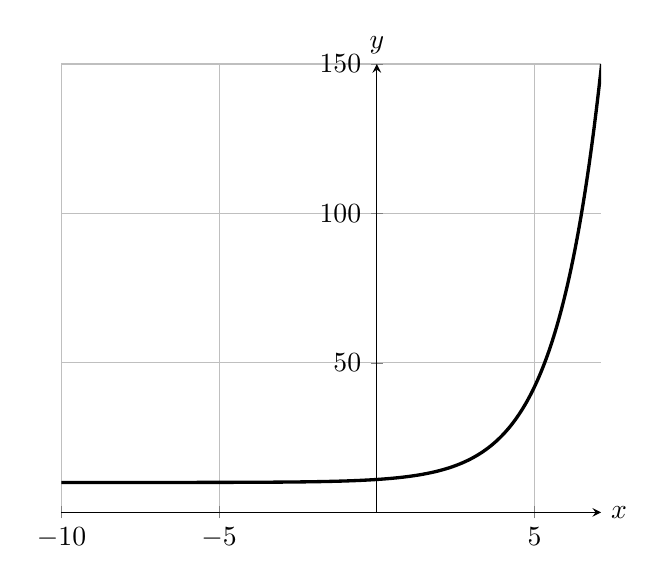
\begin{tikzpicture}
	\begin{axis}
	[ymin=0,ymax=150, axis lines=center,xlabel=$x$,ylabel=$y$,every axis y 
	label/.style={at=(current axis.above origin),anchor=south},every axis x label/.style={at=(current axis.right of origin),anchor=west},
	domain=-1:2,
	ytick={50,100,150},
	yticklabels={$50$,$100$,$150$},
	xtick={-10,-5,5},
	xticklabels={$-10$,$-5$,$5$},
	ymajorgrids=true,
	grid = major
	]
	\addplot[domain=-10:7.13,very thick,smooth,samples=1000]
	{pow(2,\x)+10};
	\end{axis}
       \end{tikzpicture}
\end{minipage}
\end{center}


\end{exercise}
\end{document}